\documentclass[border=4pt]{standalone}
% Shared typography and colours for the standalone figures.
\usepackage{unicode-math}
\setmainfont{TeX Gyre Termes}
\setsansfont{TeX Gyre Heros}
\setmonofont{TeX Gyre Cursor}
\setmathfont{TeX Gyre Termes Math}
\usepackage{tikz}
\usetikzlibrary{arrows.meta,positioning,calc,decorations.pathreplacing}
\usepackage{pgfplots}
\pgfplotsset{compat=1.18}
\definecolor{elemA}{HTML}{1F5FA8}
\definecolor{elemB}{HTML}{B8461B}
\definecolor{elemC}{HTML}{2E7D32}
\definecolor{elemD}{HTML}{6A4C93}
\definecolor{frameline}{HTML}{555555}

\usepgfplotslibrary{groupplots}
\begin{document}
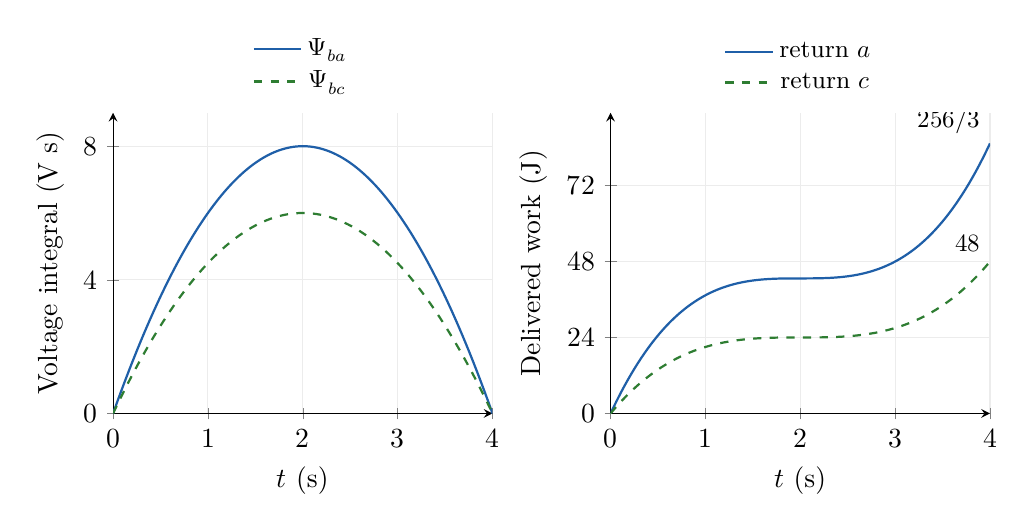
\begin{tikzpicture}
\begin{groupplot}[group style={group size=2 by 1,horizontal sep=1.5cm},width=6.4cm,height=5.4cm,
 xmin=0,xmax=4,samples=201,xlabel={$t$ (s)},axis lines=left,grid=major,grid style={gray!15},
 legend style={draw=none,font=\small,at={(.5,1.03)},anchor=south}]
\nextgroupplot[ylabel={Voltage integral (V s)},ymin=0,ymax=9,ytick={0,4,8}]
\addplot[elemA,thick,domain=0:4] {-4*(x^2/2-2*x)};\addlegendentry{$\Psi_{ba}$}
\addplot[elemC,thick,dashed,domain=0:4] {-3*(x^2/2-2*x)};\addlegendentry{$\Psi_{bc}$}
\nextgroupplot[ylabel={Delivered work (J)},ymin=0,ymax=95,ytick={0,24,48,72}]
\addplot[elemA,thick,domain=0:4] {16*(x^3/3-2*x^2+4*x)};\addlegendentry{return $a$}
\addplot[elemC,thick,dashed,domain=0:4] {9*(x^3/3-2*x^2+4*x)};\addlegendentry{return $c$}
\node[anchor=south east,font=\small] at (axis cs:4,{256/3}) {$256/3$};
\node[anchor=south east,font=\small] at (axis cs:4,48) {$48$};
\end{groupplot}
\end{tikzpicture}
\end{document}
